\question{13.9}{
    Een consumentenorganisatie wil onderzoeken hoe de samenhang is tussen de ouderdom van automobielen en de jaarlijkse kosten voor onderhoud.
    Voor auto's van het merk Inceatti zijn tien exemplaren in het onderzoek betrokken geweest.
    Dit leverde de volgende gegevens:
    \begin{center}
        \begin{tabular}{ccc}
            \toprule
                {\bfseries Auto nummer} & {\bfseries Leeftijd (\boldmath$X$)} & {\bfseries Onderhoudskosten (\boldmath$Y$)} \\
                & {\bfseries in jaren } & {\bfseries in de laatste $12$ maanden} \\ 
            \cmidrule{1-1} \cmidrule{2-2} \cmidrule{3-3} 
                $A$ & $1,6$ & $450$ \\
                $B$ & $6,8$ & $930$ \\
                $C$ & $5,1$ & $670$ \\
                $D$ & $7,2$ & $920$ \\
                $E$ & $3,5$ & $640$ \\
                $F$ & $6,2$ & $900$ \\
                $G$ & $9,4$ & $1440$ \\
                $H$ & $5,5$ & $760$ \\
                $I$ & $8,0$ & $1260$ \\
                $J$ & $2,7$ & $530$ \\
            \midrule
                Totaal & $56,0$ & $8500$ \\
            \bottomrule
        \end{tabular}
    \end{center}
    Verder zijn de volgende sommaties gegeven:
    \[ 
        \sum x_i = 56, \sum y_i = 8 500, \sum x_i^2=367,24, \sum y_i^2 = 8 102 000 \text{ en } \sum x_iy_i=54 132.
    \]
}
\begin{enumerate}[label=(\alph*)]
    \item Bereken de regressielijn waardoor de onderhoudsuitgaven worden verklaard uit de leeftijd.
    \answer{
        De regressielijn is van de vorm $Y = a + b\cdot X$, waarbij we de regressieco\"effici\"enten $a$ en $b$ bepalen aan de hand van 
        \begin{align*}
            b &= \frac{\overline{xy} - \overline{x} \cdot \overline{y}}{\overline{x^2} - (\overline{x})^2} \\
            a &= \overline{y} - b \cdot \overline{x}
        \end{align*}
        Veel van het rekenwerk is al gegeven in de opdracht.
        Het is dus niet nodig de hele rekentabel uit te werken.
        We hoeven alleen maar de sommaties om te zetten naar gemiddeldes door te delen door de steekproefgrootte $n = 10$.
        Dit geeft als gemiddeldes
        \[ 
            \overline{x} = 5,6, \quad \overline{y} = 850, \quad \overline{x^2} = 36,724, \quad \overline{y^2} = 810 200, \quad \overline{xy} = 5413,2.
        \]

        We hebben nu alle grootheden die benodigd zijn om de co\"effici\"enten van de regressielijn $Y = a + b \cdot X$ te kunnen bepalen:
        \begin{align*}
            b   &= \frac{\overline{xy} - \overline{x} \cdot \overline{y}}{\overline{x^2} - (\overline{x})^2} \\
                &= \frac{5413,2 - 5,6 \cdot 850}{36,724 - (5,6)^2} \\
                &= \frac{653,2}{5,364} \approx 121,7748 \\
            a   &= \overline{y} - b \cdot \overline{x} \\
                &= 850 - 121,7748 \cdot 5,6 \\
                &\approx 168,0611.
        \end{align*}
        De formule van de regressielijn behorende bij deze steekproef is dus gelijk aan $Y = 168,0611+121,7748\cdot X$. 
        
        \begin{center}
            \resizebox{0.9\textwidth}{!}{
                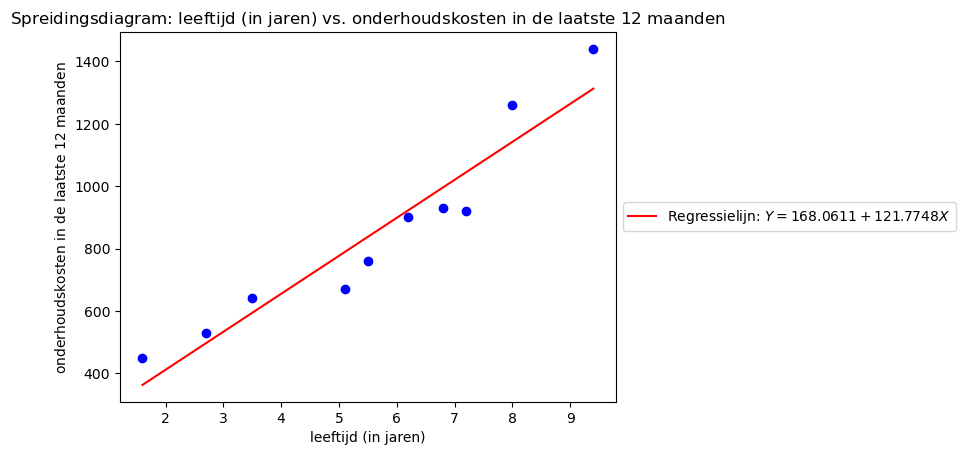
\includegraphics{opg13.9.png}
            }
        \end{center}
    }

    \item Bereken op basis van de gegevens van (a) een $95\%$-voorspellingsinterval voor de onderhoudskosten van een willekeurige auto van tien jaar oud.
    \answer{
        De eerste stap is om de puntschatting voor $Y$ te bepalen aan de hand van de regressielijn $Y = 168,0611+121,7748X$ door $X = 10$ in te vullen.
        Dit geeft ons een puntschatting van $y_0 = 168,0611 + 121,7748 \cdot 10 \approx 1385,8091$.
        Daarnaast kunnen we de standaardafwijking $\sigma$ van de storingsterm $\varepsilon$ schatten:
        \begin{align*}
            s_{\varepsilon} &= \sqrt{ \frac{n}{n-2} \cdot \left( \overline{y^2} - a \cdot \overline{y} - b \cdot \overline{xy} \right) } \\ 
                            &= \sqrt{ \frac{10}{8} \cdot \left( 810200 - 168,0611 \cdot 850 - 121,7748 \cdot 5413,2 \right) } \\ 
                            &\approx 100,9746 
        \end{align*}

        Vervolgens kunnen we een puntschatting berekenen van de standaardafwijking van $Y$ gegeven $X = x_0$:
        \begin{align*}
            s_{f}   &= s_{\varepsilon} \cdot \sqrt{ 1 + \frac{1}{n} \cdot \left( 1 + \frac{(x_0 - \overline{x})^2}{(\overline{x^2} - \overline{x}^2)} \right) } \\
                    &= 100,9746 \cdot \sqrt{ 1 + \frac{1}{10} \cdot \left( 1 + \frac{(10 - 5,6)^2}{(36,724 - 5,6^2)} \right) } \\
                    &\approx 122,0468 
        \end{align*}

        Omdat we de standaardafwijkingen geschat hebben en de storingstermen normaal verdeeld zijn, moeten we werken met de $t$-verdeling met $df = n - 2 = 8$ vrijheidsgraden.
        De grenswaarde die hoort bij een betrouwbaarheidsniveau $\alpha = 0,05$ is gelijk aan
        \[
        t = \invt(\text{opp} = 1 - \alpha / 2; \text{df} = n - 2) = \invt(\text{opp} = 0,975; \text{df} = 8) \approx 2,3060
        \]
        Het $95\%$-betrouwbaarheidsinterval voor de gemiddelde $Y$ voor gegeven $X = x_0$ kan dus worden beschreven door
        \begin{align*}
            &[y_0 - t \cdot s_{{f}}; y_0 - t \cdot s_{{f}}] \\ 
            &=[1385,8091 - 2,3060 \cdot 122,0468, 1385,8091 + 2,3060 \cdot 122,0468] \\ 
            &\approx [1104,3688, 1667,2494] 
        \end{align*}

        Met $95\%$ betrouwbaarheid liggen de onderhoudskosten in de laatste $12$ maanden van een willekeurige Inceatti auto van $10$ jaar oud tussen ongeveer $1104$ en $1667$ euro.
    }

    \item Veronderstel eens dat de hier bedoelde regressielijn exact bekend zou zijn, bijvoorbeeld omdat een alomvattend onderzoek naar onderhoudskosten heeft plaatsgevonden waarbij alle $50 000$ Inceatti-auto's die in Nederland rondrijden, betrokken waren.
    Dit bleek een regressielijn op te leveren met $\alpha=320$ en $\beta=130$.
    Verder geldt voor de storingsterm $\sigma_{\varepsilon} = 65$.
    Geef hiermee een $99\%$-voorspellingsinterval voor het bedrag aan jaarlijkse onderhoudskosten voor een willekeurige Inceatti-auto van tien jaar oud.
    \answer{
        Het daadwerkelijke verband tussen de variabelen ``leeftijd (in jaren)'' ($X$) en ``onderhoudskosten in de laatste $12$ maanden'' ($Y$) is gelijk aan
        \begin{align*}
            Y = \alpha + \beta \cdot X + \varepsilon = 320 + 130 \cdot X + \varepsilon,
        \end{align*}
        waarbij de storingsterm $\varepsilon \sim N(0, 65)$.

        Voor een willekeurige Inceatti-auto van tien jaar oud geldt dus $X = 10$.
        Dat betekent dat we $Y$ volledig kunnen beschrijven met alleen de storingsterm $\varepsilon$ als kansvariabele:
        \begin{align*}
            Y = 320 + 130 \cdot 10 + \varepsilon = 1620 + \varepsilon.
        \end{align*}

        We kunnen $Y$ dus als een kansvariabele zien die normaal verdeeld is met verwachtingswaarde $\mu = 1620$ en standaardafwijking $\sigma=65$.
        Omdat we een \SI{99}{\percent}-voorspellingsinterval willen bepalen (dus het betrouwbaarheidsniveau $\alpha = 0,01$), geldt dat $z_{\alpha/2} = \invnorm(\text{opp}=1 - \alpha/2) = \invnorm(\text{opp}=0,995) \approx 2,5758$.

        Het \SI{99}{\percent}-voorspellingsinterval voor een volgende uitkomst van $Y$ wordt dan gegeven door
        \begin{align*}
                    &[\mu - z_{\alpha/2} \cdot \sigma; \mu + z_{\alpha/2} \cdot \sigma] \\
            =       &[1620 - 2,5758 \cdot 65; 1620 + 2,5758 \cdot 65] \\
            \approx &[1452,5711; 1787,4289]
        \end{align*}
        Voor een willekeurige Inceatti-auto van tien jaar oud zullen met \SI{99}{\percent} zekerheid de onderhoudskosten in de laatste $12$ maanden tussen de $1452$ en $1788$ euro bedragen.
        \begin{center}
            \resizebox{0.9\textwidth}{!}{
                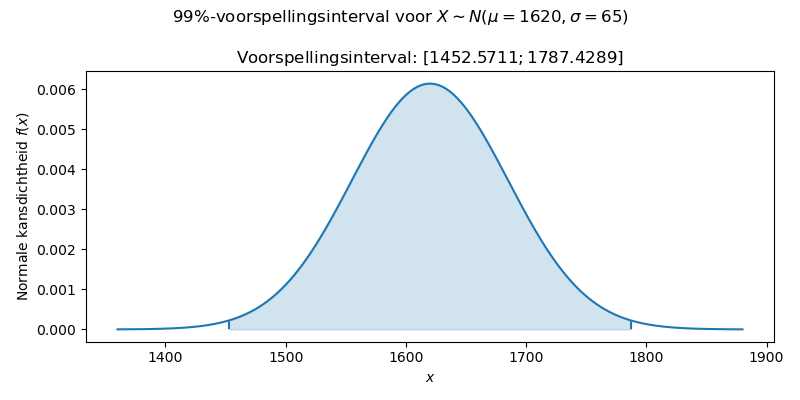
\includegraphics{opg13.9c.png}
            }
        \end{center}
    }
\end{enumerate}